\subsection{Ejercicios de construcción - Pappus}


\begin{section-exercise}
    Aplicar el teorema de Pappus, sabiendo que
    \begin{tabular}{|c|c|c|}
        \hline
        B & C & A\\\hline
        D & E & F\\
        \hline \hline
        &&\\
        \hline
    \end{tabular}
    \vspace{-0.4cm}
    \begin{figure}[H]
        \centering
        \begin{tikzpicture}[scale = 1.5]
    \clip(-4.11,-1.15) rectangle (2.65,6.29);
    \draw [line width=1.2pt,domain=-4.11:2.65] plot(\x,{(--4.44--0.34*\x)/1.11});
    \draw [line width=1.2pt,domain=-4.11:2.65] plot(\x,{(--4.35-0*\x)/2.46});
    \begin{scriptsize}
        \fill [color=black] (-2.53,3.23) circle (2.0pt);
        \draw[color=black] (-2.57,3.63) node {$A$};
        \fill [color=black] (-1.42,3.56) circle (2.0pt);
        \draw[color=black] (-1.41,3.98) node {$B$};
        \fill [color=black] (0.88,4.27) circle (2.0pt);
        \draw[color=black] (0.85,4.6) node {$C$};
        \fill [color=black] (-2.6,1.77) circle (2.0pt);
        \draw[color=black] (-2.59,1.42) node {$D$};
        \fill [color=black] (-0.14,1.77) circle (2.0pt);
        \draw[color=black] (-0.13,1.42) node {$E$};
        \fill [color=black] (0.98,1.77) circle (2.0pt);
        \draw[color=black] (0.99,1.4) node {$F$};
    \end{scriptsize}
\end{tikzpicture}
    \end{figure}
\end{section-exercise}
\vspace{-4cm}
\begin{section-exercise}
    Aplicar el teorema de Pappus, sabiendo que
    \begin{tabular}{|c|c|c|}
        \hline
        A & C & B\\\hline
        E & D & F\\
        \hline \hline
        &&\\
        \hline
    \end{tabular}
    \vspace{-0.4cm}
    \begin{figure}[H]
        \centering
        \begin{tikzpicture}[scale = 1.5]
    \clip(-4.08,-0.64) rectangle (2.26,5.84);
    \draw [line width=1.2pt,domain=-4.08:2.26] plot(\x,{(--3.59-0.46*\x)/1.18});
    \draw [line width=1.2pt,domain=-4.08:2.26] plot(\x,{(--1.58-0*\x)/0.9});
    \begin{scriptsize}
        \fill [color=black] (-2.29,3.92) circle (2.0pt);
        \draw[color=black] (-2.31,4.22) node {$A$};
        \fill [color=black] (-1.1,3.46) circle (2.0pt);
        \draw[color=black] (-1.1,3.77) node {$B$};
        \fill [color=black] (0.06,3.01) circle (2.0pt);
        \draw[color=black] (0.04,3.26) node {$C$};
        \fill [color=black] (-2.6,1.77) circle (2.0pt);
        \draw[color=black] (-2.59,1.51) node {$D$};
        \fill [color=black] (-1.7,1.77) circle (2.0pt);
        \draw[color=black] (-1.7,1.51) node {$E$};
        \fill [color=black] (0.2,1.76) circle (2.0pt);
        \draw[color=black] (0.2,1.49) node {$F$};
    \end{scriptsize}
\end{tikzpicture}
    \end{figure}
\end{section-exercise}

\begin{section-exercise}
    Aplicar el teorema de Pappus, sabiendo que
    \begin{tabular}{|c|c|c|}
        \hline
        A & B & C\\\hline
        F & D & E\\
        \hline \hline
        &&\\
        \hline
    \end{tabular}
    \vspace{-2cm}
    \begin{figure}[H]
        \centering
        \begin{tikzpicture}[scale = 1.5]
    \clip(-4.11,-1.15) rectangle (2.65,6.29);
    \draw [line width=1.2pt,domain=-4.11:2.65] plot(\x,{(--4.44--0.34*\x)/1.11});
    \draw [line width=1.2pt,domain=-4.11:2.65] plot(\x,{(--4.35-0*\x)/2.46});
    \begin{scriptsize}
        \fill [color=black] (-2.53,3.23) circle (2.0pt);
        \draw[color=black] (-2.57,3.63) node {$A$};
        \fill [color=black] (-1.42,3.56) circle (2.0pt);
        \draw[color=black] (-1.41,3.98) node {$B$};
        \fill [color=black] (0.88,4.27) circle (2.0pt);
        \draw[color=black] (0.85,4.6) node {$C$};
        \fill [color=black] (-2.6,1.77) circle (2.0pt);
        \draw[color=black] (-2.59,1.42) node {$D$};
        \fill [color=black] (-0.14,1.77) circle (2.0pt);
        \draw[color=black] (-0.13,1.42) node {$E$};
        \fill [color=black] (0.98,1.77) circle (2.0pt);
        \draw[color=black] (0.99,1.4) node {$F$};
    \end{scriptsize}
\end{tikzpicture}
    \end{figure}
    \vspace{-2cm}
\end{section-exercise}

\begin{section-exercise}
    Aplicar el teorema de Pappus, sabiendo que
    \begin{tabular}{|c|c|c|}
        \hline
        C & A & B\\\hline
        D & F & E\\
        \hline \hline
        &&\\
        \hline
    \end{tabular}
    \begin{figure}[H]
        \centering
        \begin{tikzpicture}[scale = 1.5]
    \clip(-3.97,0.64) rectangle (4.46,5);
    \draw [line width=1.2pt,domain=-3.97:4.46] plot(\x,{(--4.3--0.16*\x)/1.2});
    \draw [line width=1.2pt,domain=-3.97:4.46] plot(\x,{(--3.6--0.03*\x)/2});
    \begin{scriptsize}
        \fill [color=black] (-2.53,3.23) circle (2.0pt);
        \draw[color=black] (-2.57,3.63) node {$A$};
        \fill [color=black] (-1.33,3.39) circle (2.0pt);
        \draw[color=black] (-1.33,3.8) node {$B$};
        \fill [color=black] (-0.34,3.53) circle (2.0pt);
        \draw[color=black] (-0.36,3.86) node {$C$};
        \fill [color=black] (-2.9,1.75) circle (2.0pt);
        \draw[color=black] (-2.88,1.4) node {$D$};
        \fill [color=black] (-0.89,1.78) circle (2.0pt);
        \draw[color=black] (-0.89,1.44) node {$E$};
        \fill [color=black] (3.25,1.85) circle (2.0pt);
        \draw[color=black] (3.25,1.49) node {$F$};
    \end{scriptsize}
\end{tikzpicture}
    \end{figure}
\end{section-exercise}


\newpage
\subsection{Ejercicios de perspectiva - Desargues}

\begin{multicols}{2}
    [
        \begin{section-exercise}
            Encuentre, con la ayuda de una regla, el punto y la recta para los cuales los triángulos \theTriangle{ABC} y \theTriangle{XYZ} están en perspectiva.
        \end{section-exercise}
    ]

    \begin{figure}[H]
        \centering
        
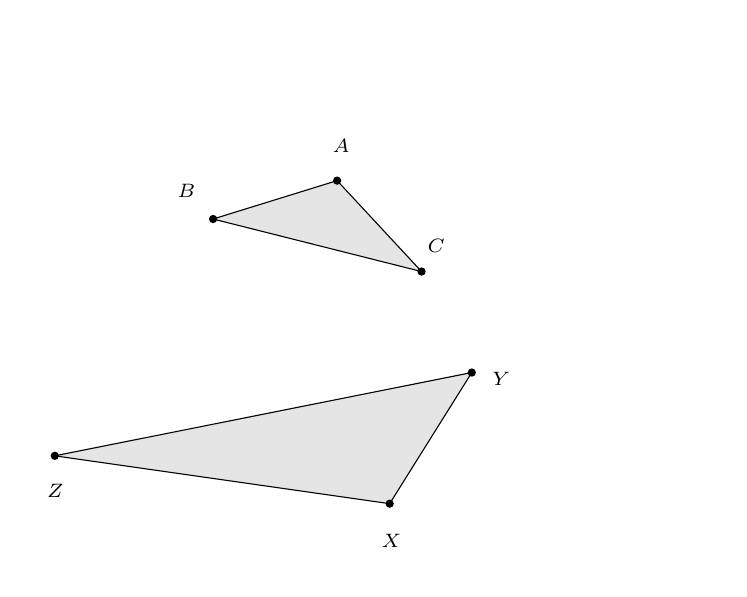
\begin{tikzpicture}[scale = 0.75]
    \clip(-7.11,-1.61) rectangle (4.59,7.55);
    \fill[fill=black,fill opacity=0.1] (-3.97,4.31) -- (-1.87,4.96) -- (-0.44,3.42) -- cycle;
    \fill[fill=black,fill opacity=0.1] (-6.65,0.3) -- (-0.98,-0.51) -- (0.41,1.71) -- cycle;
    \draw (-3.97,4.31)-- (-1.87,4.96);
    \draw (-1.87,4.96)-- (-0.44,3.42);
    \draw (-0.44,3.42)-- (-3.97,4.31);
    \draw (-6.65,0.3)-- (-0.98,-0.51);
    \draw (-0.98,-0.51)-- (0.41,1.71);
    \draw (0.41,1.71)-- (-6.65,0.3);
    \begin{scriptsize}
        \fill [color=black] (-1.87,4.96) circle (2.0pt);
        \draw[color=black] (-1.8,5.54) node {$A$};
        \fill [color=black] (-3.97,4.31) circle (2.0pt);
        \draw[color=black] (-4.42,4.78) node {$B$};
        \fill [color=black] (-0.44,3.42) circle (2.0pt);
        \draw[color=black] (-0.19,3.85) node {$C$};
        \fill [color=black] (-0.98,-0.51) circle (2.0pt);
        \draw[color=black] (-0.95,-1.14) node {$X$};
        \fill [color=black] (-6.65,0.3) circle (2.0pt);
        \draw[color=black] (-6.64,-0.29) node {$Z$};
        \fill [color=black] (0.41,1.71) circle (2.0pt);
        \draw[color=black] (0.91,1.6) node {$Y$};
    \end{scriptsize}
\end{tikzpicture}
    \end{figure}

    \begin{figure}[H]
        \centering
        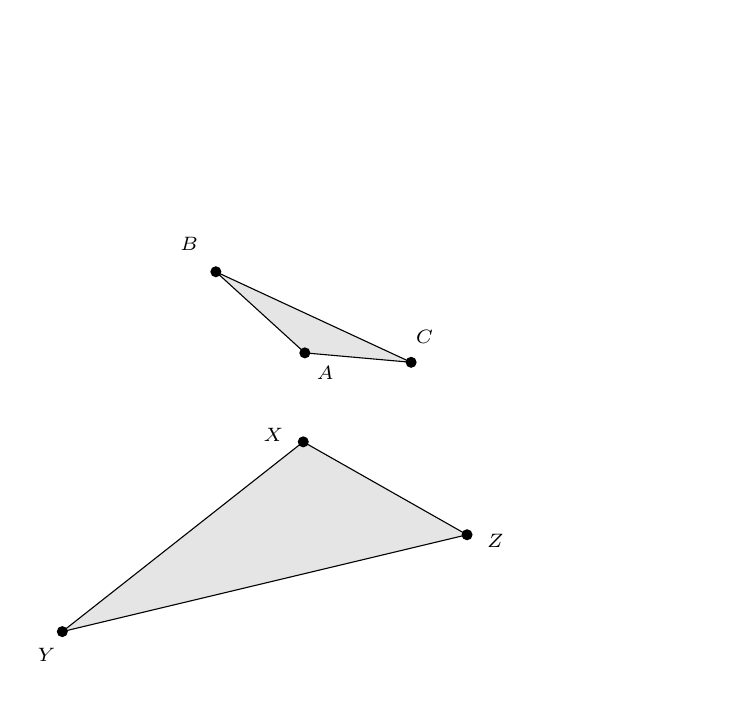
\begin{tikzpicture}[scale = 1]
    \clip(-5.5,-1.15) rectangle (3.12,7.27);
    \fill[fill=black,fill opacity=0.1] (-3.11,4.17) -- (-1.98,3.14) -- (-0.63,3.02) -- cycle;
    \fill[fill=black,fill opacity=0.1] (-5.06,-0.4) -- (-2,2.01) -- (0.08,0.83) -- cycle;
    \draw (-3.11,4.17)-- (-1.98,3.14);
    \draw (-1.98,3.14)-- (-0.63,3.02);
    \draw (-0.63,3.02)-- (-3.11,4.17);
    \draw (-5.06,-0.4)-- (-2,2.01);
    \draw (-2,2.01)-- (0.08,0.83);
    \draw (0.08,0.83)-- (-5.06,-0.4);
    \begin{scriptsize}
        \fill [color=black] (-1.98,3.14) circle (2.0pt);
        \draw[color=black] (-1.72,2.88) node {$A$};
        \fill [color=black] (-3.11,4.17) circle (2.0pt);
        \draw[color=black] (-3.45,4.52) node {$B$};
        \fill [color=black] (-0.63,3.02) circle (2.0pt);
        \draw[color=black] (-0.46,3.34) node {$C$};
        \fill [color=black] (-2,2.01) circle (2.0pt);
        \draw[color=black] (-2.38,2.1) node {$X$};
        \fill [color=black] (-5.06,-0.4) circle (2.0pt);
        \draw[color=black] (-5.26,-0.7) node {$Y$};
        \fill [color=black] (0.08,0.83) circle (2.0pt);
        \draw[color=black] (0.44,0.75) node {$Z$};
    \end{scriptsize}
\end{tikzpicture}
    \end{figure}

    \begin{figure}[H]
        \centering
        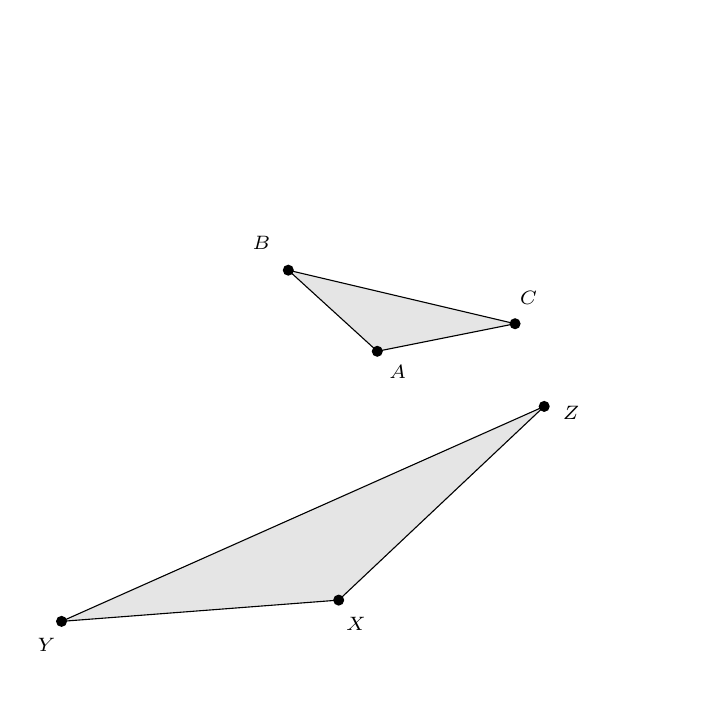
\begin{tikzpicture}[scale = 1]
    \clip(-6.42,-1.07) rectangle (2.01,7.25);
    \fill[fill=black,fill opacity=0.1] (-3.11,4.17) -- (-1.98,3.14) -- (-0.23,3.49) -- cycle;
    \fill[fill=black,fill opacity=0.1] (-5.99,-0.29) -- (-2.47,-0.02) -- (0.14,2.44) -- cycle;
    \draw (-3.11,4.17)-- (-1.98,3.14);
    \draw (-1.98,3.14)-- (-0.23,3.49);
    \draw (-0.23,3.49)-- (-3.11,4.17);
    \draw (-5.99,-0.29)-- (-2.47,-0.02);
    \draw (-2.47,-0.02)-- (0.14,2.44);
    \draw (0.14,2.44)-- (-5.99,-0.29);
    \begin{scriptsize}
        \fill [color=black] (-1.98,3.14) circle (2.0pt);
        \draw[color=black] (-1.72,2.88) node {$A$};
        \fill [color=black] (-3.11,4.17) circle (2.0pt);
        \draw[color=black] (-3.45,4.52) node {$B$};
        \fill [color=black] (-0.23,3.49) circle (2.0pt);
        \draw[color=black] (-0.06,3.82) node {$C$};
        \fill [color=black] (-2.47,-0.02) circle (2.0pt);
        \draw[color=black] (-2.25,-0.32) node {$X$};
        \fill [color=black] (-5.99,-0.29) circle (2.0pt);
        \draw[color=black] (-6.18,-0.59) node {$Y$};
        \fill [color=black] (0.14,2.44) circle (2.0pt);
        \draw[color=black] (0.48,2.36) node {$Z$};
    \end{scriptsize}
\end{tikzpicture}
    \end{figure}

    \begin{figure}[H]
        \centering
        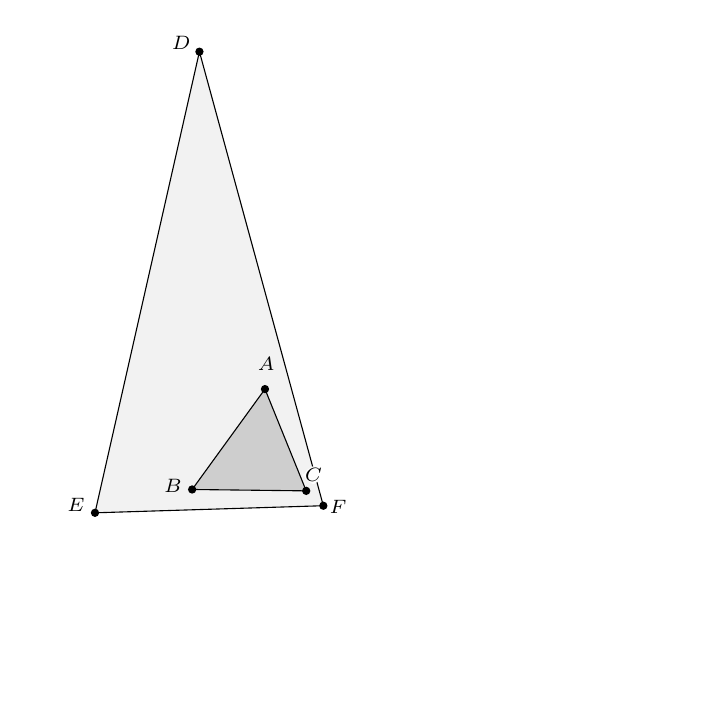
\begin{tikzpicture}[scale = 0.125]
    \clip(-22.59,-26.1) rectangle (44.94,41.07);
    \fill[fill=black,fill opacity=0.15] (1.52,4.35) -- (-5.88,-5.85) -- (5.71,-5.99) -- cycle;
    \fill[fill=black,fill opacity=0.05] (-5.14,38.63) -- (-15.75,-8.22) -- (7.45,-7.5) -- cycle;
    \draw (1.52,4.35)-- (-5.88,-5.85);
    \draw (-5.88,-5.85)-- (5.71,-5.99);
    \draw (5.71,-5.99)-- (1.52,4.35);
    \draw (-5.14,38.63)-- (-15.75,-8.22);
    \draw (-15.75,-8.22)-- (7.45,-7.5);
    \draw (7.45,-7.5)-- (-5.14,38.63);
    \begin{scriptsize}
        \fill [color=black] (1.52,4.35) circle (12pt);
        \draw[color=black] (1.64,6.88) node {$A$};
        \fill [color=black] (-5.88,-5.85) circle (12pt);
        \draw[color=black] (-7.84,-5.47) node {$B$};
        \fill [color=black] (5.71,-5.99) circle (12pt);
        \draw[color=black] (6.44,-4.39) node[fill = white, rounded corners = 5pt, inner sep=0.8pt] {$C$};
        \fill [color=black] (-5.14,38.63) circle (12pt);
        \draw[color=black] (-7,39.51) node {$D$};
        \fill [color=black] (-15.75,-8.22) circle (12pt);
        \draw[color=black] (-17.67,-7.39) node {$E$};
        \fill [color=black] (7.45,-7.5) circle (12pt);
        \draw[color=black] (8.95,-7.63) node {$F$};
    \end{scriptsize}
\end{tikzpicture}
    \end{figure}

\end{multicols}